
\chapter{Обзор работы}
\label{chapter1}

В этой главе представлен общий обзор работы: уточнены цели и объяснены термины и понятия, присутствующие в решении задачи. Также произведен обзор имеющихся результатов и сформулирована постановка задачи.

\section{Недоминирующая сортировка}

В данном разделе представлено определение недоминирующей сортировки и необходимые для ее понимания понятия. Также рассмотрены недостатки рассмотренных алгоритмов, и обоснована необходимость их резрешения.

\subsection{Определение}

Недоминирующая сортировка {---} это процедура, которая ранжирует множество точек в многомерном пространстве $R^n$.
Если описывать неформально, то ее задача определить, какие точки "лучше" других. При этом допускается, что две точки
могут быть одинаково "хорошими". На рисунке ~\ref{nds} подставлен пример недоминирующей сортировки конкретных точек.

\begin{figure}[!h]
\begin{center}
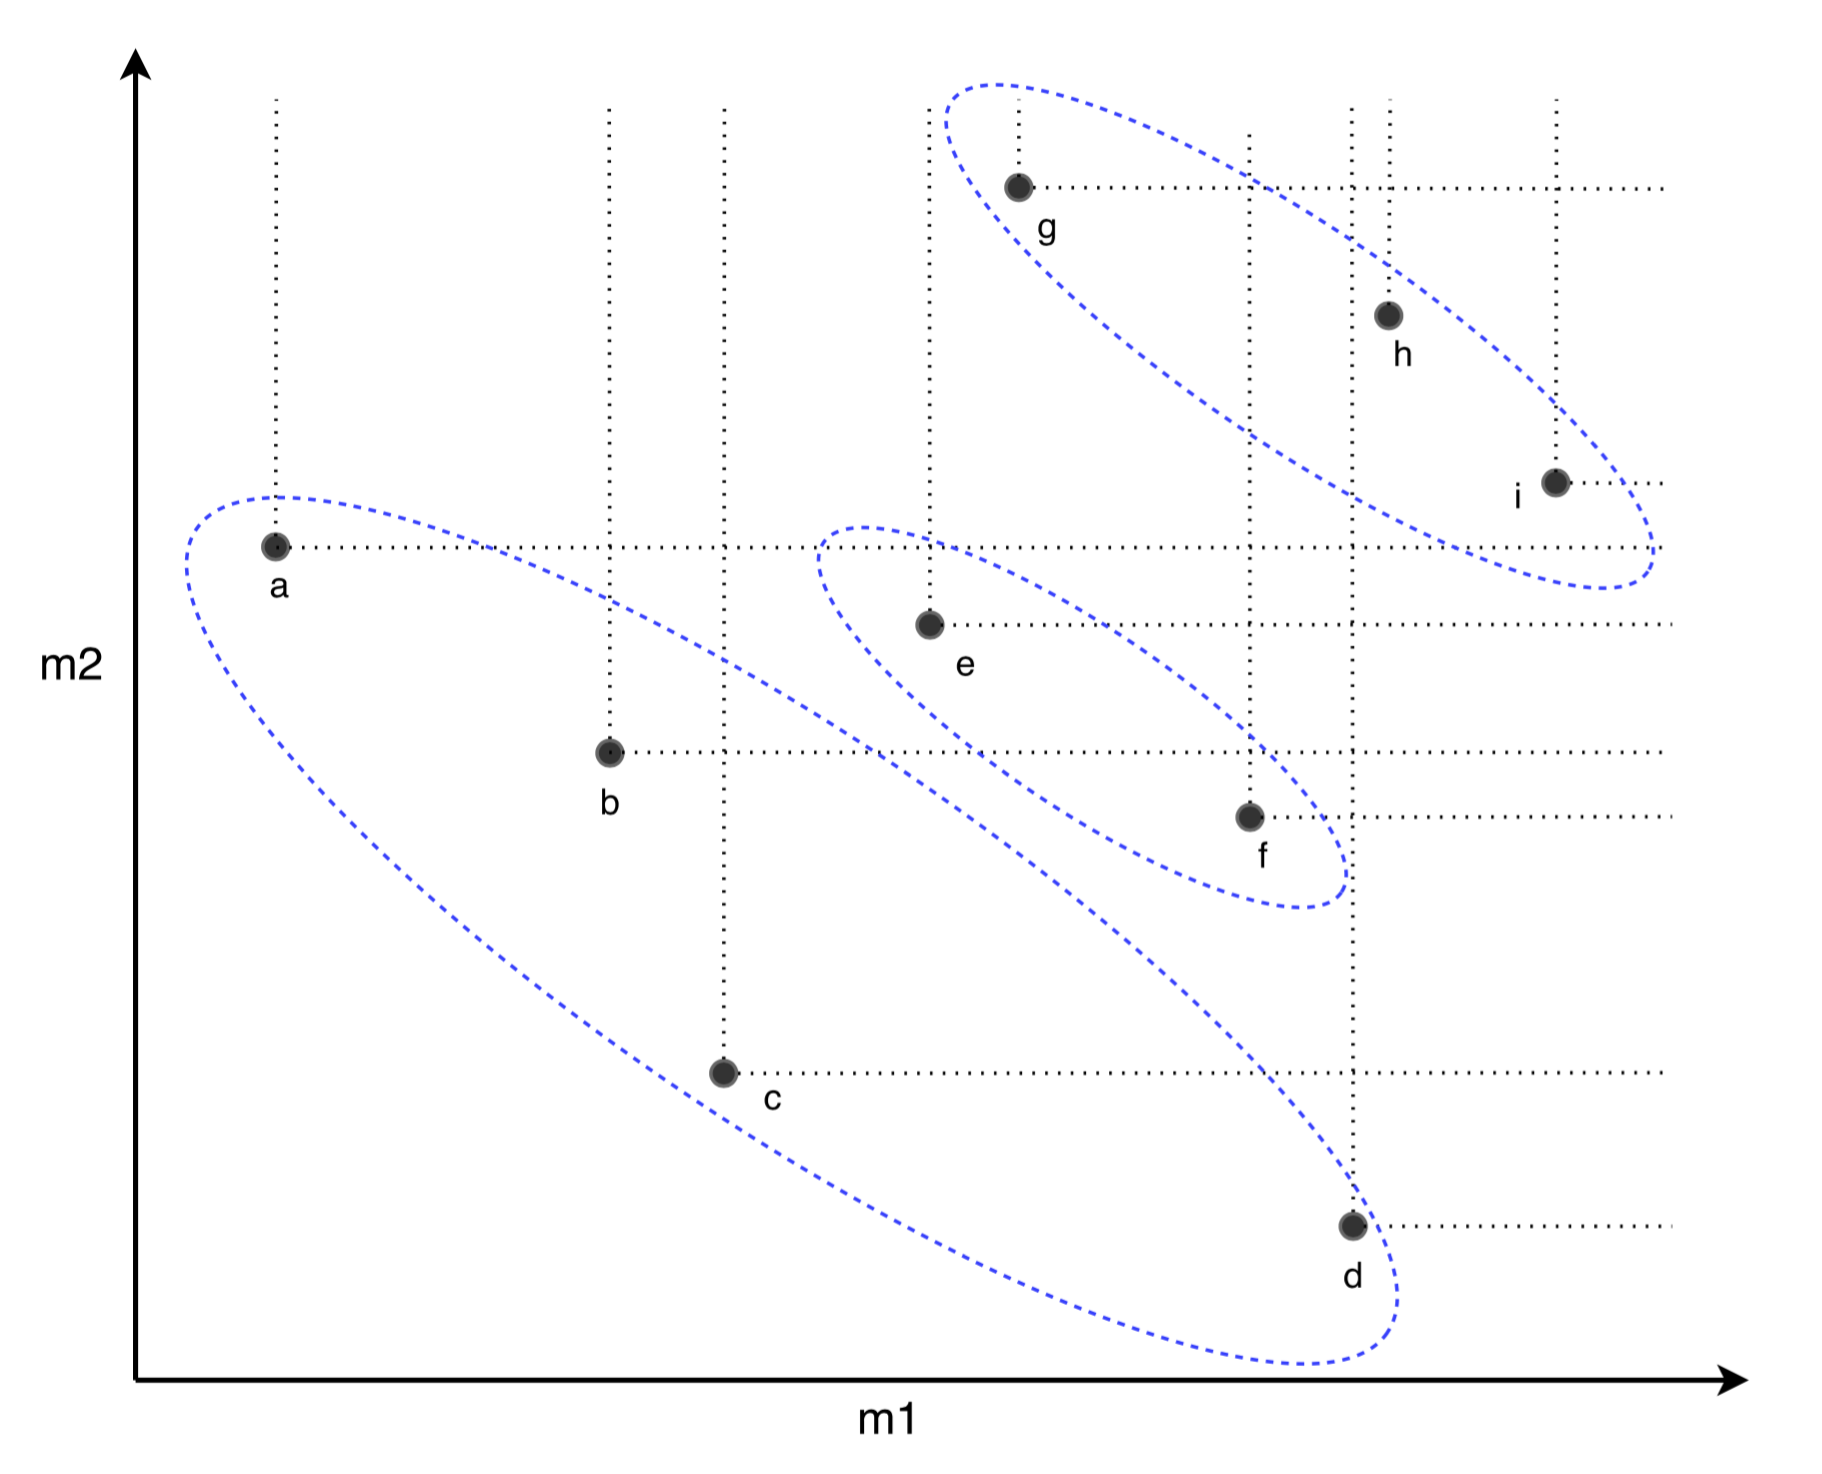
\includegraphics[width=9cm]{pic/non_dominated_sort.png}
\caption{На рисунке представлен пример недоминирующей сортировки для точек \{a,b,c,d,e,f,g,h,i\}.
Точки \{a,b,c,d\} имеют ранг 0, \{e,f\} {---} 2, \{g,h,i\} {---} 3.}
\label{nds}
\end{center}
\end{figure}

Для того, чтобы сформулировать определение недоминирующей сортировки, сначала надо определить, какие точки мы считаем
"лучше" других. Для этого введем определение доминирования одной точки другой.

\textit{Определение.} В $M$-мерном пространстве, точка $A = (a_1,...,a_M)$ доминирует точку $B = (b_1,...,b_M)$
 тогда и только тогда, когда для всех $1 \leq i \leq M$ выполняется неравенство $a_i\leq b_i$, и существует такое $j$,
 что $a_j < b_j$.

"Лучшими" в данном контексте будут считаться точки, которые не доминируются ни одной другой точкой или, другими словами,
лежащие на Парето-фронте. Однако часто бывают не только точки с Парето-фронта, но и другие "хорошие" точки. Таким
образом мы приходим к определению процедуры недоминирующей сортировки.

\textit{Определение.} Недоминирующая сортировка множества точек $S$ в $M$-мерном пространстве {---} это процедура, которая
назначает всем точкам из $S$ ранг. Все точки, которые не доминируются ни одной точкой из $S$ имеют ранг ноль. Точка
имеет ранг $i+1$, если максимальный ранг среди доминирующих её точек равен $i$.

\subsection{Применение и актуальность}

Самый яркий пример применения процедуры недоминирующей сортировки {---} алгоритмы многокритериальной оптимизации, особенно эволюционные алгоритмы. Последние на каждой итерации генерируют множество потенциальных решений и оценивают каждое решение по всем критериям. Если критериев $M$, то получается набор из $N$ $M$-мерных векторов, где $N$ {---} число потенциальных решений. И эволюционному алгоритму на каждой итерации надо отобрать лучшие решения, для чего и требуется недоминирующая сортировка.

Если каждый критерий для каждого потенциального решения считается достаточно долго, то время выполнения недоминирующей сортировки становится неважным, так как асимптотика каждой итерации алгоритма зависит в основном от асимптотики времени подсчета критериев. Однако гораздо чаще встречаются задачи, в которых подсчет каждого критерия занимает время значительно меньшее, чем время, необходимое для недоминирующей сортировки. Именно в таких случаях ускорение алгоритмов недоминирующей сортировки ускорит время выполнения итерации алгоритма, а следовательно и время выполнения всего алгоритма.

В настоящее время существует много алгоритмов недоминирующей сортировки, но каждый из них имеет свои слабые стороны. Это означает, что существует возможность сделать алгоритм, который мог бы заранее предсказывать, время работы какого алгоритма на данном наборе точек будет меньше, и выбирать оптимальный. Более того, есть возможность совместить идеи разных алгоритмов в одном, который всегда будет работать не хуже существующих. Такие возможности делают проблему ускорения алгоритмов недоминирующей сортировки еще более актуальной.

\section{Анализ существующих алгоритмов}

В данном разделе будут рассмотрена история развития алгоритмов недоминирующей сортировки. Особое внимание будет уделено самым эффективным алгоритмам, которые применяются для гибридизации в данной работе. Они будут рассмотрены наиболее подробно.

\subsection{Наивные алгоритмы}

Опишем самый наивный алгоритм недоминирующей сортировки. Он перебирает все пары точек и сравнивает их по всем критериям. После этого он присваивает нулевой ранг тем из них, которые не доминируются ни одной  другой точкой и отбрасывает их из множества. Данная процедура повторяется, пока в множестве остаются точки. Причем на каждом новом шаге присваивается новое значение ранга, на единицу больше, чем на предыдущем шаге. Рассмотрим время работы данного наивного алгоритма. Пусть $N$ {---} это число точек, а $M$ {---} размерность пространства. Тогда сравнение всех пар точек по $M$ критериям займет $O(MN^2)$, а всего шагов алгоритма будет не больше, чем максимальное число рангов {---} $N$. Таким образом, время работы данного алгоритма не превышает $O(MN^3)$, причем эта оценка достигается в худшем случае при максимальном числе рангов в сортируемом множестве.

В работе Кунга и др. \cite{Kung} предлагается алгоритм определения множества недоминируемых точек, при этом его вычислительная сложность составляет $O(N log^{M-1} N)$. Этот алгоритм можно использовать для выполнения недоминирующей сортировки аналогично вышеописанному алгоритму. Сначала в множестве $S$ алгоритм Кунга находит множество точек с рангом $0$. Затем алгоритм Кунга запускается на оставшемся множестве точек, и получившемуся множеству точек присваивается ранг $1$. Процесс выполняется до тех пор, пока имеются точки, которым не присвоен ранг. Описанная процедура в худшем случае выполняется за $O(N^2 log^{M-1} N)$, если максимальный ранг точки равен $O(N)$.

Также существует много других алгоритмов, асимптотика которых равна $O(MN^2)$, например, алгоритм ENS Жанга и др.~\cite{Zhang}.

\subsection{Алгоритм ``Разделяй и Властвуй''}

Йенсен \cite{Jensen} впервые предложил алгоритм недоминирующей сортировки с вычислительной сложностью $O(N log^{M-1} N)$. Однако, как корректность, так и оценка сложности алгоритма доказывалась в предположении, что никакие две точки не имеют совпадающие значения ни в какой размерности. Однако довольно часто алгоритмы оптимизации работают с дискретными критериями, поэтому совпадение разных решений по одному критерию может быть довольно частым событием. Устранить указанный недостаток оказалось достаточно трудной задачей — первой успешной попыткой сделать это, насколько известно исполнителю данной НИР, является работа Фортена и др. \cite{Forton}. Исправленный (или, согласно работе, «обобщенный») алгоритм корректно работает во всех случаях, и во многих случаях его время работы составляет $O(N log^{M-1} N)$, но единственная оценка времени работы для худшего случая, доказанная в работе \cite{Jensen}, равна $O(N^2M)$. Наконец, в работе Буздалова и др. \cite{Buzdalov} предложены модификации алгоритма из работы \cite{Jensen}, которые позволили доказать в худшем случае также и оценку $O(N log^{M-1} N)$, не нарушая корректности работы алгоритма.

Опишем подробнее алгоритм Буздалова и др., так как он будет использоваться в гибридном алгоритме, разрабатываемом в данной работе. Основная идея алгоритма {---} принцип ``разделяй и властвуй'', основанный на разбиении исходного множества на несколько меньших множеств и решении задачи на этих множествах. Алгоритм на каждом шаге находит медиану множества по последнему критерию и делит его на три подмножества элементов, меньших медианы по последнему критерию, больших и равных ей. Далее алгоритм рекурсивно запускается на каждом подмножестве с некоторыми промежуточными вычислениями. На рисунке ~\ref{fast_pic} схематически изображена идея алгоритма на основе метода ``разделяй и властвуй''.

\begin{figure}[!h]
\begin{center}
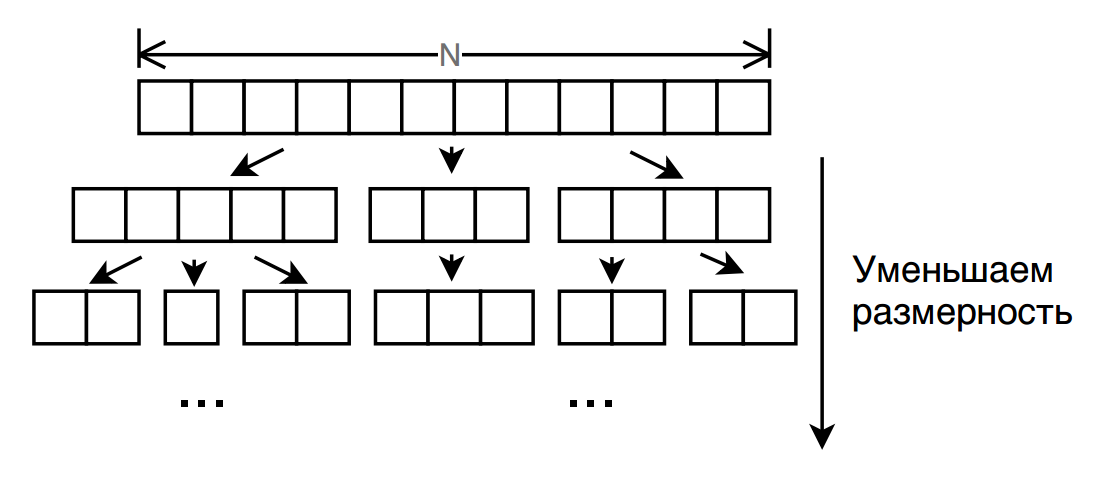
\includegraphics[width=9cm]{pic/fast_pic.png}
\caption{Идея алгоритма на основе метода ``разделяй и властвуй''.}
\label{fast_pic}
\end{center}
\end{figure}

Рассмотрим подробнее процедуры, использующиеся в алгоритме Буздалова. Основными из них являются процедуры $NDHelperA$, $NDHelperB$ и $SplitBy$. Первая как раз и представляет собой основной алгоритм на множестве $S$, которое дается ему на вход. Однако она может также присвоить ранги точкам так, чтобы они не стали меньше, чем ранги, которые эти точки имели до исполнения процедуры. Также данная процедура сравнивает точки только по первым $k$ критериям. Эти дополнения необходимы для возможности корректного рекурсивного вызова данной процедуры. Алгоритм Буздалова, по сути, заключается в том, что расставляет всем точкам множества $S$ ранг ноль, а затем запускает процедуру $NDHelperA$ c аргументами $S$ и $M$.

Процедура $NDHelperA$ не работает с размерностями меньше $2$, так как для них есть более эффективные алгоритмы, которые она и запускает при необходимости.

Псевдокод $NDHelperA$ представлен на листинге ~\ref{nd-helper-a}.

\begin{algorithm}
\begin{algorithmic}[1]
\Procedure{NDHelperA}{S, k}
    \If{$|S| < 2$} \Return
    \ElsIf{$|S| = 2$}
        \State $\{s^{(1)}, s^{(2)}\} \gets S$
        \If{$s_{1:k}^{(1)} \prec s_{1:k}^{(2)}$}
            \State $\textsc{rank}(s^{(2)}) \gets \max\{\textsc{rank}(s^{(2)}), \textsc{rank}(s^{(1)})+1\}$
        \EndIf
    \ElsIf{$k = 2$}
        \State \textsc{SweepA}($S$)
    \ElsIf{$|\{ s_k | s \in S \}| = 1$}
        \State \textsc{NDHelperA}(S, $k - 1$)
    \Else
        \State{$L, M, H \gets \textsc{SplitBy}(S, \text{median}\{s_k | s \in S\}, k)$}
        \State{\textsc{NDHelperA}($L$, $k$)}
        \State{\textsc{NDHelperB}($L$, $M$, $k - 1$)}
        \State{\textsc{NDHelperA}($M$, $k - 1$)}
        \State{\textsc{NDHelperB}($L \cup M$, $H$, $k - 1$)}
        \State{\textsc{NDHelperA}($H$, $k$)}
    \EndIf
\EndProcedure
\end{algorithmic}
\caption{Процедура \textsc{NDHelperA}. Она присваивает ранги точкам из $S$ по первым $k$ рангам.}
\label{nd-helper-a}
\end{algorithm}

Следующая процедура $NDHelperB$ запускается между рекурсивными запусками $NDHelperA$ на трех подмножествах. Задача этой процедуры {---} расставить минимально возможные ранги точек для подмножества, на котором сейчас запустится $NDHelperA$. Простая имплементация данной процедуры могла бы перебрать все пары точек из множества точек с уже проставленными рангами и точек, на которых сейчас запустится $NDHelperA$, и проставить каждой точке из  второго множества ранг, на единицу большие, чем максимальный ранг точки с уже проставленным рангом, которая ее доминирует. Однако это работало бы квадратичное время по размеру подмножеств, поэтому данная процедура также использует принцип ``разделяй и властвуй'' и при расстановке минимальных рангов также разбивает множества на более мелкие и запускается на них рекурсивно.

Более подробно процедура $NDHelperB$ описана в псевдокоде на листинге ~\ref{nd-helper-b}.

\begin{algorithm}
\begin{algorithmic}[1]
\Procedure{NDHelperB}{L, H, k}
    \If{$L = \{\}$ or $H = \{\}$} \Return
    \ElsIf{$|L| = 1$ or $|H| = 1$}
        \ForAll{$h \in H$, $l \in L$}
            \If{$l_{1:k} \preceq h_{1:k}$}
                \State $\textsc{rank}(h) \gets \max\{\textsc{rank}(h), \textsc{rank}(l) + 1\}$
            \EndIf
        \EndFor
    \ElsIf{$k = 2$}
        \State \textsc{SweepB}($L$, $H$)
    \ElsIf{$\max\{l_k | l \in L\} \le \min\{h_k | h \in H\}$}
        \State \textsc{NDHelperB}($L$, $H$, $k - 1$)
    \ElsIf{$\min\{l_k | l \in L\} \le \max\{h_k | h \in H\}$}
        \State{$m \gets \text{median}\{ s_k | s \in L \cup H \}$}
        \State{$L_1, M_1, H_1 \gets \textsc{SplitBy}(L, m, k)$}
        \State{$L_2, M_2, H_2 \gets \textsc{SplitBy}(H, m, k)$}
        \State{\textsc{NDHelperB}($L_1$, $L_2$, $k$)}
        \State{\textsc{NDHelperB}($L_1$, $M_2$, $k - 1$)}
        \State{\textsc{NDHelperB}($M_1$, $M_2$, $k - 1$)}
        \State{\textsc{NDHelperB}($L_1 \cup M_1$, $H_2$, $k - 1$)}
        \State{\textsc{NDHelperB}($H_1$, $H_2$, $k$)}
    \EndIf
\EndProcedure
\end{algorithmic}
\caption{Процедура \textsc{NDHelperB}. Она подгоняет ранги точек из $H$
         используя первые $k$ критериев, сравнивая их с точками из $L$.}
\label{nd-helper-b}
\end{algorithm}

Последняя процедура, которую стоит упомянуть для описания алгоритма Буздалова и др. {---} процедура разбиения множеств $SplitBy$. Она работает за линейное время по размеру множества, которое она разбивает и делит его на три множества: точки, большие $m$ по критерию $k$, равные $m$ и меньшие $m$. В каждом получившемся подмножестве сохраняется порядок точек, который был в оригинальном множестве.

Процедура $SplitBy$ описана на листинге ~\ref{split-by}.

\begin{algorithm}
\begin{algorithmic}[1]
\Procedure{SplitBy}{S, m, k}
    \State{$L \gets \{ s \in S | s_k < m \}$}
    \State{$M \gets \{ s \in S | s_k = m \}$}
    \State{$H \gets \{ s \in S | s_k > m \}$}
    \State{\Return $L$, $M$, $H$}
\EndProcedure
\end{algorithmic}
\caption{Процедура разбиения. В каждом подмножестве используется такой же
         порядок точек, как и до разбиения.}
\label{split-by}
\end{algorithm}

\subsection{Алгоритм Роя и др.}

Большой интерес представляет алгоритм Роя $Best~Order~Sort~(BOS)$ \cite{Roy}, который в отличии вышеупомянутых не
использует метод разделяй и властвуй. Его вычислительная сложность $O(MNlogM+MN^2)$. В лучшем случае алгоритм
работает за $O(MNlogM)$, что лучше алгоритма предложенного Буздаловым и др. Однако в худшем случае его асимптотика
совсем другая {---} $O(MN^2)$. Авторами алгоритма не было проведено более точных исследований по его времени работы.

\subsection{Алгоритм Густавссона и др.}

Большой интерес представляет алгоритм Густавссона и Сиберфильдта ENS-NDT \cite{Gustavsson}, который в отличии вышеупомянутых не использует метод разделяй и властвуй. Его вычислительная сложность на случайно сгенерированных независимых точек равна $O(N^{1.43})$. Однако в худшем случае алгоритм работает за квадратичное время $O(MN^2)$.

Опишем основную идею этого алгоритма и приведем псевдокоды основных методов. Более детальное описание можно найти в статье \cite{Gustavsson}.
Подробное описание необходимо в данной работе для понимания оптимизаций, модификации алгоритма и для понимания итогового гибридного алгоритма.

Алгоритм Густавссона и Сиберфильдта ENS-NDT относится к группе Efficient Non-dominated Sort. Еще одним представилем этой группы является алгоритм ENS-BS (Efficient Non-dominated Sort Binary Strategy), скорость работы которого сильно ухудшается с ростом количества точек. Алгоритм ENS-NDT справляется и с большим количеством точек и с точками большой размерности в общем случае.

Недоминирующее дерево (NDTree) основано на Bucket k-d дереве. Bucket k-d дерево - это вид бинарного дерева, где хранятся точки k-мерного пространства. Каждая вершина дерева ассоциирована с одной размерностью. Листья имеют так называемый bucket size - максимальное количество точек, которое может содержать лист, если появляется необходимость добавить больше точек, вершина делится на две. Медианы, которые используются при построении дерева преподсчитаны для всех вершин для соответствующих им размерностям. Далее, если точка по рассматриваемой в данной вешине координате меньше, чем медианное значение, то процесс добавления продолжается в левом ребенке-вершине, если больше - то в правом. Точки, чьи координаты равны медианному значению, добавляются в левого или правого ребенка, в зависимости от настроек k-d дерева. Новые вершины ассоциированы с новым критерием, отличным от родительской вершины, обычно используется следующий критерий, то есть критерий родительской вершины + 1 или первый критерий, если родительский параметр ассоциирован с максимальной размерностью.  На рисунке ~\ref{ndt_explanation} подставлена иллюстрация bucket k-d дерева. Вершина A ассоциирована с критерием X, вершины B и C ассоциирована с критерием Y, вершины D и E ассоциирована с критерием X снова, bucket size представленной на рисунке структуры равен трем. Также, чтобы избежать создания слишком большого количества уровней, NDTree имеет параметр максимальной глубины. Это означает, что если достигнута максимальная глубина, то параметры максимального количества точек в вершине ингорируется.

\begin{figure}[!h]
\begin{center}
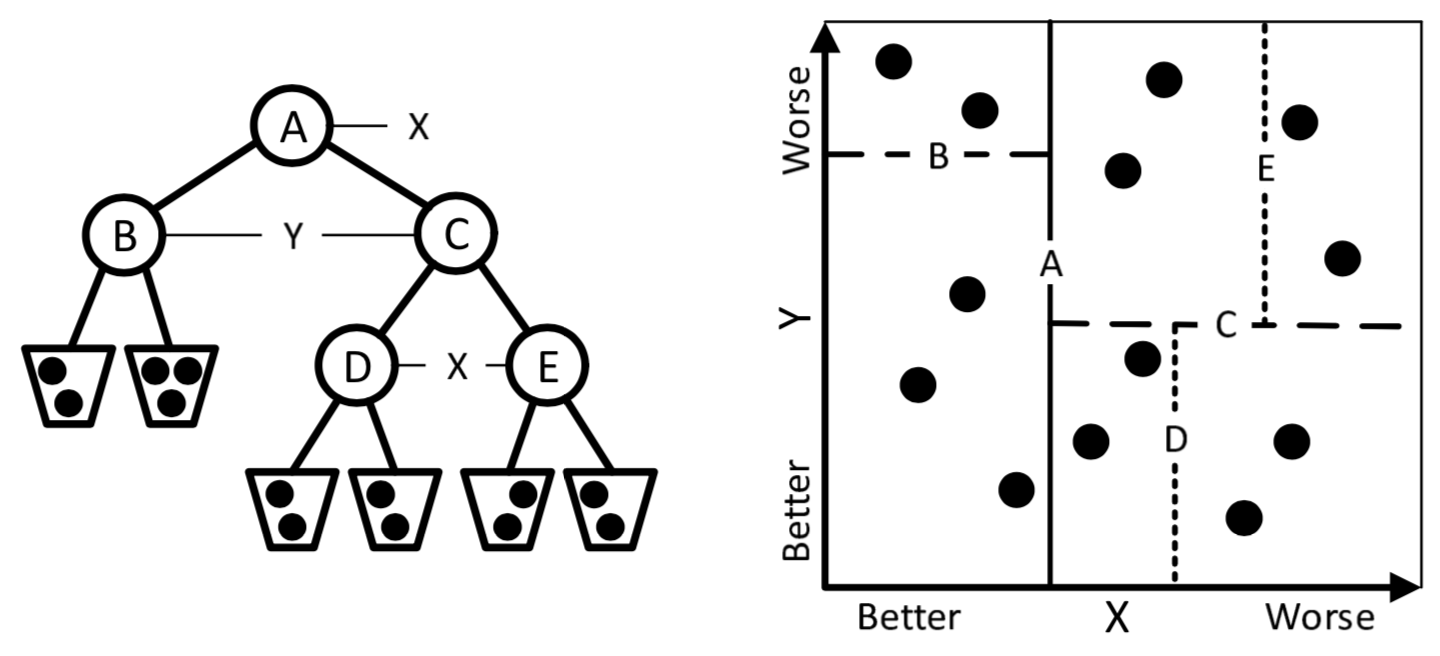
\includegraphics[width=15cm]{pic/ndt_explanation.png}
\caption{На рисунке представлена иллюстрация внутреннего устройства структуры Bucket k-d tree. Слева изображена структура, справа точки на плоскости, по которым получена структура.}
\label{ndt_explanation}
\end{center}
\end{figure}

NDTree использует преподсчитанное split множество, где все возможные медианные значения преподсчитаны до того, как они потребуются. Это отличается от стандартной реализации bucket k-d дерева, в котором обычно значение считается в момент переполнения максимального допустимого количества точек в вершине. Это становится возможно сделать, потому что мы знаем множество точек для сортировки заранее. Основное преимущество использования split дерева заключается в том, что девево остается сбалансированным, что значительно улучшает производительность поиска. Split множество удобно хранить в виде дерева, похожем на финальное недоминирующее дерево.

Для выполнения недоминирующей сортировки следует поддерживать отдельное дерево для каждого ранга. На рисунке ~\ref{ndtree_original} представлено схематическое представление структуры использующейся в недоминирующей сортировке.

\begin{figure}[!h]
\begin{center}
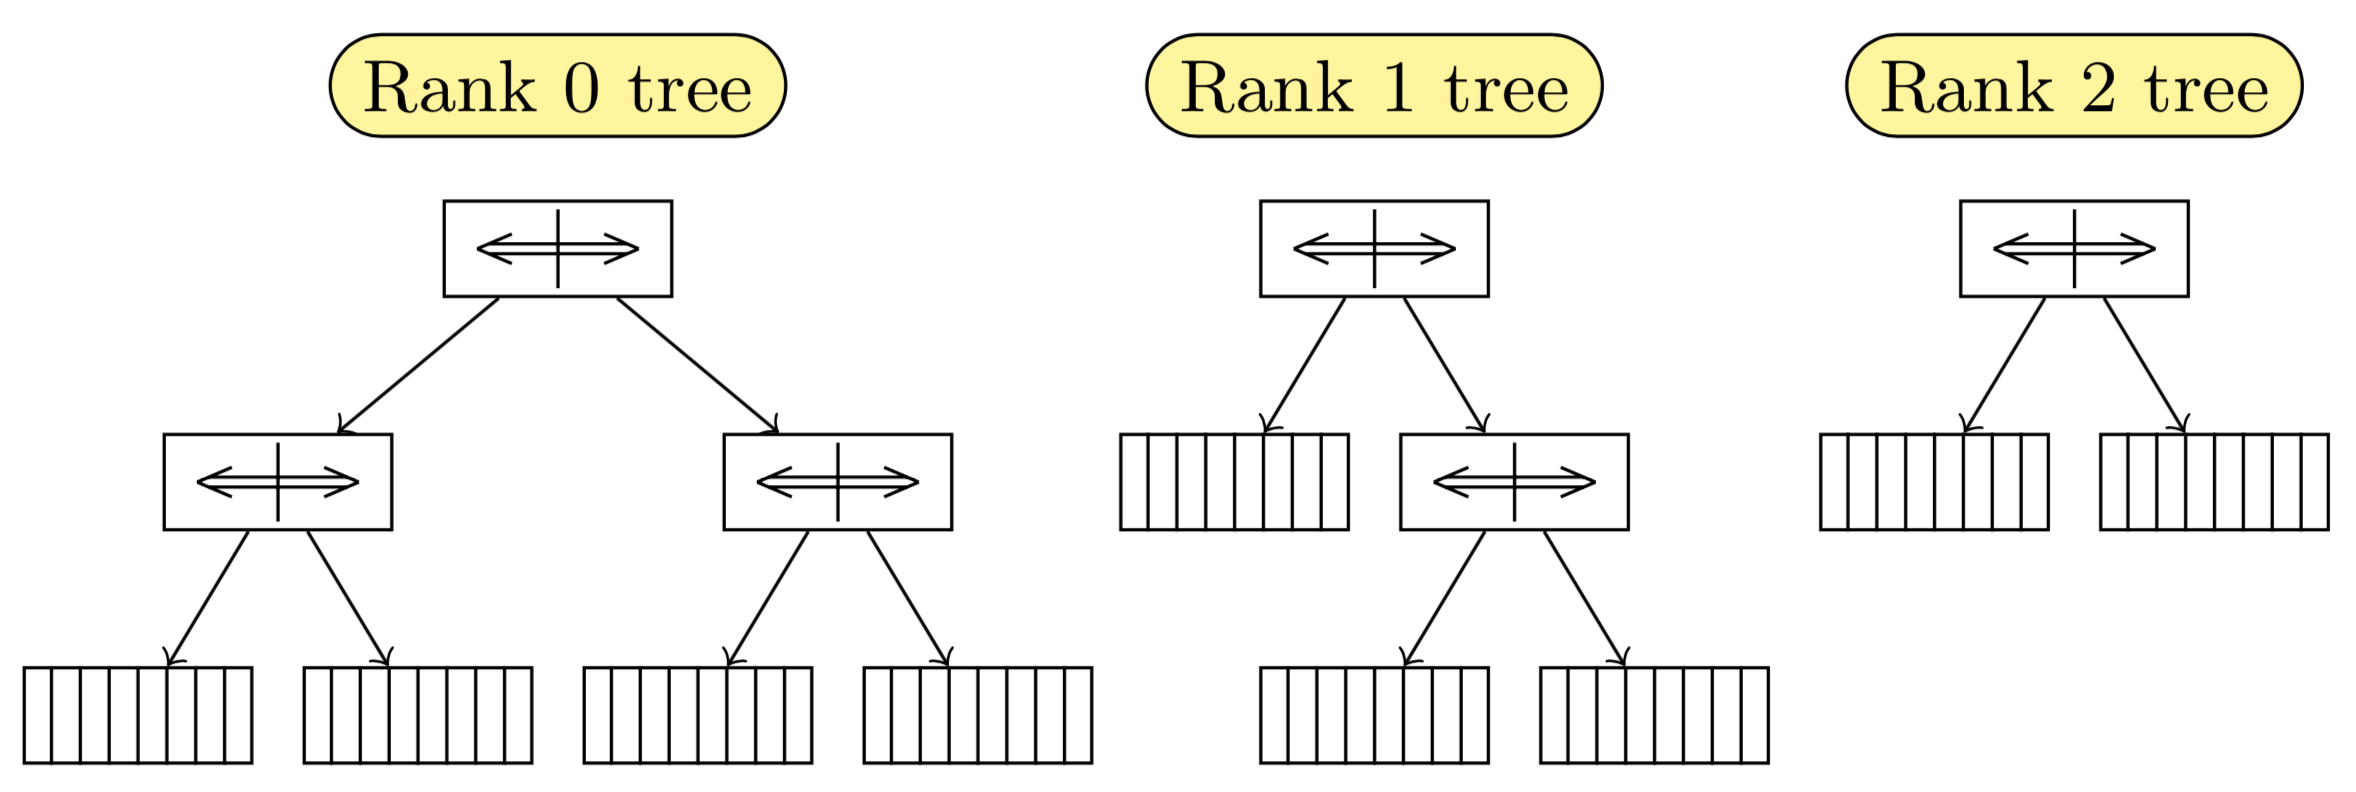
\includegraphics[width=15cm]{pic/ndtree_original.png}
\caption{Структура деревьев для алгоритма ENS-NDT. Каждое дерево ассоциировано с отдельным рангом.}.
\label{ndtree_original}
\end{center}
\end{figure}

Для выполнения недоминирующей сортировки следует выполнить следующие действия:
\begin{enumerate}
\item Создать split структуру для всех точек.
\item Осуществить лексикографическую сортировку.
\item Перебираем точки в лексикографическом порядке.
    \begin{enumerate}
    \item Определяем ранг.
    \item Добавляем в соответствующее рангу дерево.
    \end{enumerate}
\end{enumerate}

Ниже представлен псевдокод на листинге ~\ref{procedure_end_ndt} основного метода недоминирующей сортировки, который принимает в качестве аргументов множество точек P, M - размерность и B - порог, то есть максимальное количество точек в вершине. Для получения split структуры используется функция CreateSplits, которая на вход получает множество точек, порог и размерность M-1, размерность M-ая игнорируется, так как ранее множество точек было лексикографически отсортировано. Лексикографическая сортировка выбрана еще потому, что она позвоняет уменьшить число сравнений.

Следующим шагом будет создание множества $\mathcal{F}$ и $\mathcal{T}$ на строчке 4-6, $\mathcal{F}$ - это ранжированное множество точек, $\mathcal{T}$ - множество деревьев для каждого ранга, в каждом дереве ни одна точка не доминирует другую точку в том же дереве. Точка $P_1$ добавляется в оба множества с рангом один, так как ни одна другая точка не может доминировать первую из-за лексикографической сортировки. Главный цикл на строке 8 определяет ранги точек и добавляет их в структуру.

\begin{algorithm}
\begin{algorithmic}[1]
\Procedure{ENS-NDT}{P, M, B}
    \State{$S \gets CreateSplits(P, M-1,B)$}
    \State{$P \gets Sort(P, a^M \prec b^M, ..., a^1 \prec b^1)$}
    \State{$\mathcal{F} \gets \{\{P_1\}\}$}
    \State{$\mathcal{T} \gets \{new NDTree(S, B)\}$}
    \State{$InsertIntoNDTree(\mathcal{T}_1, P_1)$}
    \State{$j \gets 1$}
    \For{$i = 2, ..., |P|$}
        \If{$P_{i-1} \neq P_{i}$}
            \State {$j \gets FrontIndexBinarySearch(\mathcal{T}, P_i)$}
            \If{$j > |\mathcal{T}|$}
                \State{$F_j \gets 0$}
                \State{$\mathcal{T}_j \gets new NDTree(S, B)$}
            \EndIf
            \State{$InsertIntoNDTree(\mathcal{T}_j, \mathcal{P}_i,)$}
        \EndIf
        \State{$\mathcal{F}_j \gets \mathcal{F}_j \cup {P_i} $}
    \EndFor
    \State{\Return {$\mathcal{F}$}}
\EndProcedure
\end{algorithmic}
\caption{Главная процедура алгоритма ENS-NDT.}
\label{procedure_end_ndt}
\end{algorithm}

Возможная реализация CreateSplits изображена на листинге ~\ref{create_split}. Структура NDSplit похожа на NDTree, но вместо точек она хранит медианные значения. Общий подход построения сбалансированных k-d деревьев с помощью метода разделяй и властвую описан Бламом и др. ~\cite{Blum}.

Вкаратце опишем процедуру CreateSplit, TODO 

\begin{algorithm}
\begin{algorithmic}[1]
\Procedure{CreateSplit}{$P, M, B, d \gets 0$}
    \State{$o \gets 1 + (d \mod M)$}
    \State{$P \gets Sort(P, a^o \prec b^o)$}
    \State{$m \gets P_{1+\lfloor |P|/2 \rfloor}$}
    \State{$S \gets \{new NDSplit(o, m)\}$}
    \If{$|P|> B$}
        \State {$Better \gets \{P_i, i<1+\lfloor |P|/2 \rfloor\}$}
        \State {$Worse \gets \{P_i, i\geq1+\lfloor |P|/2 \rfloor\}$}
        \State {$S.BetterSplit \gets CreateSplit(Better, M, B, d+1)$}
        \State {$S.WorseSplit \gets CreateSplit(Worse, M, B, d+1)$}
    \EndIf
    \State{\Return S}
\EndProcedure
\end{algorithmic}
\caption{Пример реализации процедуры CreatSplit, которая вычисляет медианные значения для NDTree.}
\label{create_split}
\end{algorithm}

Поледней интересной для нас функцией являтся функция определения ранга точки FrontIndexBinarySearch, представленная на листинге ~\ref{rank_binary_search}. Эта процедура бинарным поиском определяет минимальное дререво в структуре $\mathcal{T}$, где ни одна точка не доминировала бы рассматриваемую. 

\begin{algorithm}
\begin{algorithmic}[1]
\Procedure{FrontIndexBinarySearch}{$\mathcal{T}, s$}
    \State{$i \gets 1$}
    \State{$j \gets |\mathcal{T}| + 1$}
    \While {$i \neq j$}
        \State {$k \gets \lfloor i + (j-i) /2 \rfloor $}
        \If {$FromntDominates(\mathcal{T}_k, s)$}
            \State {$i \gets k + 1$}
        \Else
            \State {$j \gets k$}
        \EndIf    
    \EndWhile
    \State{\Return i}
\EndProcedure
\end{algorithmic}
\caption{Процедура определения ранга точки $s$.}
\label{rank_binary_search}
\end{algorithm}

Подробное описание алгоритма ENS-NDT необходимо для понимания дальнейшей модификации и самого гибридного алгоритма.

\section{Недостатки существующих алгоритмов}

Все описанные выше алгоритмы имеют разные разные преимущества и недостатки. Алгоритм Буздалова ``разделяй и властвуй'' имеет хорошую асимптотику, даже на самых плохих входных данных. Однако алгоритм сильно замедляется с ростом размерности задачи $M$. 

Алгоритм Роя, имеет интересную идею и показал хорошие результаты на практике. Однако теоретическое время его работы пока не исследовано. 

Алгоритм Густавссона имеет хорошую асимптотику на случайно распеределенных точках в гиперкубе, но имеет квадратичную асимптотику, в описанном авторами плохом случае. 

\section{Постановка задачи}

Задача данной работы состоит в разработке нового гибридного алгоритма недоминирующей сортировки и разбивается на подзадачи:
\begin{enumerate}
	\item Выбрать наиболее подходящие для гибридизации алгоритмы.
	\item Адаптировать алгоритмы для гибридизации.
	\item Реализовать гибридный алгоритм.
	\item Настроить гибридный алгоритм для максимально эффективной работы.
\end{enumerate}
